\chapter{NLMyo : Traitement de rapports textuels par LLMs}

Dans les deux précédents chapitres, nous avons présenté \gls{impatient} un outil d'annotation et d'exploration de compte rendu de biopsie en texte libre. \gls{impatient} utilise un système à base d'ontologie et de vocabulaire standard pour détecter et annoter la présence ou l'absence d'éléments pathologiques dans les biopsies musculaires. Cependant, ce système présente certaines limites. Tout d'abord, il requiert de créer un vocabulaire standard exhaustif pour décrire les observations dans les biopsies musculaires, ce qui est un travail manuel important. De plus, le système d'annotation semi-automatique utilise un système à base de règles et de correspondance exacte des mots aux ontologies existantes. Cette correspondance exacte réduit la flexibilité du système et sa sensibilité de détection, il faut alors réaliser un travail d'annotation manuel important pour numériser les comptes rendus de biopsie. 

En fin 2022 et début 2023, les récentes avancées dans le domaine du \gls{nlp} ont permis de révolutionner la manière de traiter et d'exploiter les données sous forme de texte libre. La mise à dispositions de modèles linguistiques de grande taille (\gls{llms}, \ref{chap2_llms}) performants, accessibles et capables de suivre des instructions, ouvre la porte à la création d'outils plus performants et flexibles pour le traitement de ces comptes rendus. Ces systèmes basés sur une approche sémantique et multilingue éliminent la nécessité de définir un vocabulaire standard. Ainsi nous avons développé \gls{nlmyo} (fig \ref{fig:nlmyo_logo}), une boite à outils basée sur les \gls{llms} mettant à disposition quatre outils généralistes pour le traitement de comptes rendus médicaux: outil d'anonymisation, d'extraction d'information, de classification automatique et de création de moteurs de recherche. L'ensemble de ces outils et des modèles utilisés est représenté dans la figure \ref{fig:nlmyo_struct}.
\begin{figure}[!ht]
 \centering
 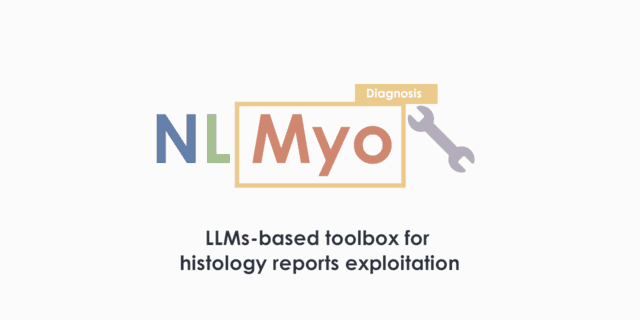
\includegraphics[width=0.5\textwidth]{figures/nlmyo_banner.png}
 \caption[Logo NLMyo]{\textbf{Logo de NLMyo}}
 \label{fig:nlmyo_logo}
\end{figure}
\begin{figure}[!ht]
 \centering
 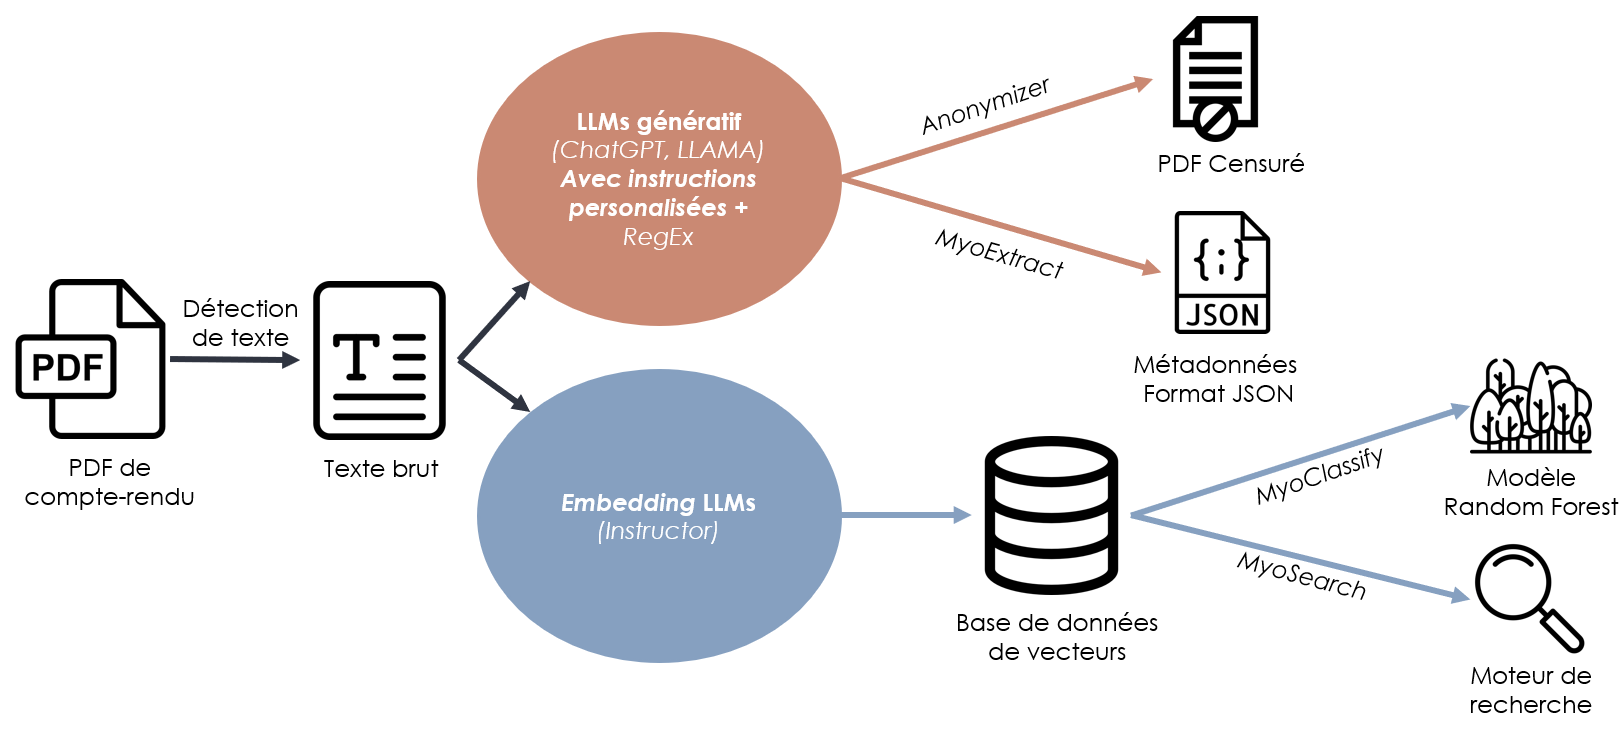
\includegraphics[width=1\textwidth]{figures/nlmyo_struct.png}
 \caption[Structure de NLMyo]{\textbf{Structure de NLMyo}. NLMyo utilise deux types de LLMs pour traiter les comptes rendus de biopsie: les modèles génératifs et les modèles d'\textit{embedding}. L'utilisation de ces deux types de modèles permet la mise à disposition de quatre outils: Anonymizer, MyoExtract, MyoClassify et MyoSerach.}
 \label{fig:nlmyo_struct}
\end{figure}
\section{\textit{Anonymizer}: un outil d'anonymisation}
Le premier outil de \gls{nlmyo} est \textit{Anonymizer}, un outil permettant de supprimer automatiquement les informations identifiantes des comptes rendus médicaux. Dans les comptes rendus de biopsie de l'Institut de Myologie de Paris que nous traitons, deux données identifiantes et personnelles sont présentes et doivent être retirées: le nom du patient (et du personnel médical) ainsi que la date de naissance du patient. Non seulement ces informations ne sont pas utiles pour les analyses subséquentes, mais de plus, par respect de la vie privée et des recommandations \gls{rgpd}, ces informations ne doivent être accessibles qu'aux professionnels en charge du patient. L'anonymisation des rapports est donc une étape essentielle avant le transfert des données, leur numérisation et leur analyse.

Afin de traiter un grand volume de rapports et d'éliminer le travail manuel nécessaire, nous avons tenté d'automatiser la tâche d'anonymisation \textit{via} deux approches: une approche traditionnelle par\gls{regex} et une approche novatrice par\gls{llms}.

\subsection{Anonymisation par RegEx}
En première intention, nous avons développé une méthode basée sur les \gls{regex} pour leur simplicité de mise en place et leur rapidité d'exécution (coûts en puissance de calcul faible). Les \gls{regex} sont des séquences de caractères capables de trouver des motifs dans un texte, par exemple toutes les lignes commençant par "Nom: ". Le tableau \ref{tab:regex} liste les \gls{regex} utilisées pour capturer les informations de noms et de dates. Les comptes rendus de biopsie sont semi-structurés. Pour la plupart, le nom du patient est facilement identifiable, car il est précédé par le préfixe: "Nom: ". Ceci est facilement représenté par la première \gls{regex} listée dans le tableau. Ensuite pour les autres cas de figure, comme les noms de famille sont souvent en majuscule et les prénoms commencent souvent par une majuscule, nous avons développé deux autres \gls{regex} pour capturer les couples de mots dont un est en majuscule et le second commence par une majuscule (ou inversement, lignes 2 et 3 du tableau). 
Ensuite, une troisième \gls{regex} a été ajoutée pour détecter les dates au format JJ-MM-AAAA ou JJ.MM.AAAA (ligne 3 du tableau). Finalement, une dernière \gls{regex} est utilisée pour essayer de trouver le numéro de biopsie dans le document afin de renommer le fichier avec un nom unique et anonyme (ligne 4 du tableau). 
\begin{table}[!ht]
\centering
\caption[Expressions régulières pour extraire les noms et les dates]{\textbf{Expressions régulières pour extraire les noms et les dates}. Trois expressions régulières sont utilisées pour détecter les noms de patients, une expression pour les dates et une expression pour les numéros de biopsie.}
\label{tab:regex}
\begin{tabular}{|l|l|l|}
\hline
\textbf{Expression régulière} & \textbf{Syntaxe} & \textbf{Exemples d'utilisation} \\ \hline
Nom patient & Nom.*: *([A-Za-zÀ-ÿ- ]+) & Nom : Pierre Laroche \\ \hline
Nom patient 2& (([A-Z][a-zÀ-ÿ-]\{3,\} ?)+ ([A-Z-]\{3,\} ?)+) & LAROCHE Pierre \\ \hline
Nom patient 3 & (([A-Z-]\{3,\} ?)+ ([A-Z][a-zÀ-ÿ-]\{3,\} ?)+) & Pierre André LAROCHE \\ \hline
Date & ([(.]?[0-9]\{1,2\}[./][0-9]\{1,2\}[./][0-9]\{1,4\}[().]?) & 07/04/1994, 07.05.18 \\ \hline
N° Biopsie & ([0-9]\{3,8\}[-/]?[0-9]\{0,3\}) & 7377-07, 1234/56 \\ \hline
\end{tabular}
\end{table}
\begin{figure}[!ht]
 \centering
 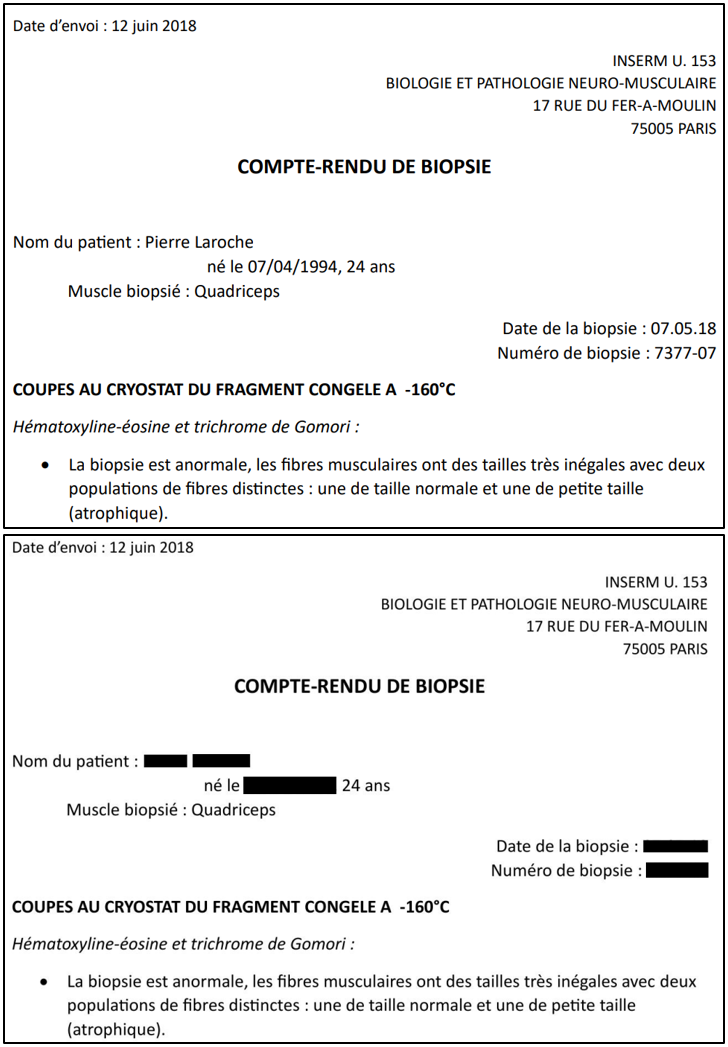
\includegraphics[width=0.8\textwidth]{figures/regex.png}
 \caption[Exemple anonymisation RegEx]{\textbf{Exemple d'anonymisation d'un compte rendus fictif de biopsie avec la méthode RegEx}. En haut le rapport à l'état brut, en bas le rapport censuré. On observe que le nom, le numéro de biopsie et deux dates ont été censurées. Cependant la date d'envoi "12 juin 2018" n'a pas été censurée.}
 \label{fig:regex}
\end{figure}

La figure \ref{fig:regex} présente les résultats de la technique d'anonymisation par \gls{regex} sur l'entête d'un rapport factice de patient, mais avec une structure similaire aux rapports de l'Institut de Myologie de Paris. Les noms et les dates ont été censurés correctement et la méthode a produit de bons résultats. Cependant, cette méthode est insuffisante, car elle est peu sensible (dates ou noms non censurés) et spécifique (informations considérées à tort comme des dates ou des noms). Par exemple tout en haut de l'entête, la date d'envoi "12 juin 2018" n'a pas été censurée. Le tableau \ref{tab:regex_fail} liste trois exemples de cas où cette méthode ne fonctionne pas et produit des erreurs. Il est possible de corriger ces erreurs en augmentant la somme de \gls{regex} utilisées, mais augmenter le nombre de \gls{regex} augmente aussi potentiellement le nombre de faux positifs. De plus, il n'est pas toujours possible de construire une \gls{regex} adaptée pour extraire une information précise. Nous avons alors exploré la capacité des \gls{llms} pour la recherche et l'extraction de ces informations de manière plus robuste et flexible que la méthode \gls{regex}.
\begin{table}[!ht]
\centering
\caption[Exemples de faux positifs ou faux négatifs de la méthode RegEx]{\textbf{Exemples de faux positifs ou faux négatifs de la méthode RegEx}. En fonction du cas de figure, les RegEx peuvent provoquer des faux positifs (censure d'informations excessive) ou des faux négatifs (information personnelle non censurée correctement).}
\label{tab:regex_fail}
\begin{tabularx}{\textwidth}{|l|l|l|X|}
\hline
\textbf{Texte} & \textbf{RegEx déclenchée} & \textbf{Type} & \textbf{Commentaire} \\ \hline
\textit{PAS Staining} & Nom patient 3 & Faux Positif & Nom de coloration dont la notation est confondue avec le motif "NOM Prénom" \\ \hline
\textit{Louis C. Dupont} & N/A & Faux Négatif & La présence du "C." au centre ne permet pas aux RegEx de nom de se déclencher \\ \hline
\textit{12 mars 2001} & N/A & Faux Négatif & La notation de date avec un mois en lettres ne permet pas à la RegEx de date de se déclencher \\ \hline
\textit{1996-04} & N° Biopsie & Faux Positif & La notation de date AAAA-MM déclenche la \gls{regex} de numéro de biopsie. \\ \hline
\end{tabularx}
\end{table}

\subsection{Anonymisation par LLMs}
Les \gls{llms} sont basés sur la compréhension du sens sémantique du texte tandis que les \gls{regex} sont basées sur le principe de motifs de caractères et donc sur la structure du document. L'idée de l'anonymisation par \gls{llms} est d'utiliser un modèle génératif auquel on fournit une instruction et le texte à anonymiser. L'instruction liste les informations à extraire du texte et spécifie le format de sortie. Pour intégrer ces modèles génératifs à outil d'anonymisation, nous voulons récupérer les informations extraites dans un format exploitable informatiquement, nous avons utilisé le format JSON. Le format JSON représente un dictionnaire informatique qui est utilisable par l'application pour censurer les PDF à partir des informations détectées.

\subsection{Instruction personnalisée et \textit{one-shot learning}}
Nous avons construit une instruction personnalisée en 3 parties qui intègre une méthode de \textit{one-shot learning}. Le \textit{one-shot learning} est une technique d'apprentissage qui vise à généralisation en ne donnant qu'un seul exemple d'apprentissage au modèle pour la l'apprentissage d'une nouvelle tâche. Dans l'instruction les trois parties sont: (i) la description de la tâche à effectuer (ii) un exemple de réalisation de la tâche \textit{(one-shot learning)}, (iii) le texte d'intérêt à anonymiser.
Voici un exemple d'instruction que nous utilisons pour réaliser l'extraction des noms et des dates dans les rapports:
\begin{quote}
Tu es un assistant qui extrait des informations d'un texte libre. Le format de ta réponse doit être un format JSON valide qui respecte le nom des clés fournies. Si une valeur est manquante, indique simplement N/A, n'essaie pas d'inventer. Voici la liste des informations à récupérer, les clés JSON sont indiquées entre parenthèses : nom complet (name), dates (date).

ENTRÉE :

Kendrick Lamar et Jane Clinton sont asymptomatiques. Date de naissance : 16 février 1991, numéro de biopsie : 666-77. Ce rapport a été expédié le 01.04.1991.

SORTIE :

\{"name" :["Kendrick Lamar", "Jane Clinton"], "date" : ["16 février 1991", "01.04.1991"]\}

ENTRÉE :

<texte à analyser>

SORTIE :
\end{quote}

La partie précédant le mot clé "ENTRÉE" correspond à l'instruction décrivant précisément la tâche que le modèle doit réaliser (liste des informations à extraire, format de sortie et comportement attendu). Le premier couple "ENTRÉE" et "SORTIE" correspond à un exemple de réalisation de la tâche, ce qui permet de spécifier le schéma JSON attendu au modèle (\textit{one-shot learning}). Puis le second couple "ENTRÉE", "SORTIE" correspond à l'endroit où l'on injecte notre texte d'intérêt à analyser et spécifie au modèle que l'on attend maintenant une sortie textuelle au format JSON pour l'entrée précédente.

\subsection{Exemple et comparaison à la méthode RegEx}
\begin{figure}[!ht]
 \centering
 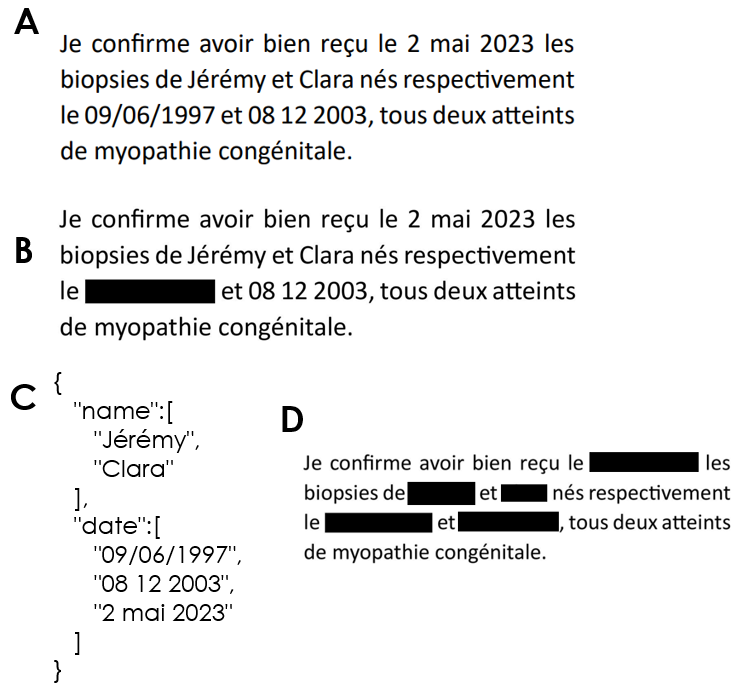
\includegraphics[width=0.8\textwidth]{figures/llms_anonym.png}
 \caption[Exemple anonymisation LLMs]{\textbf{Exemple d'anonymisation d'un courrier médical factice avec la méthode par LLMs}. \textbf{(A) }Texte brut, \textbf{(B)} Anonymisation par RegEx, \textbf{(C) }JSON brut généré par le \gls{llms} GPT-3.5-turbo (OpenAI), \textbf{(D)} Anonymisation à partir du JSON généré par \gls{llms}.}
 \label{fig:llms_anonym}
\end{figure}

Dans cet exemple (figure \ref{fig:llms_anonym}), nous avons construit un début de courrier médical factice faisant figurer des informations personnelles qui ne sont pas détectables par la méthode \gls{regex}. Les prénoms "Jérémy" et "Clara", ainsi que les dates "2 mai 2023" et "08 12 2003" n'ont pas été détectées par la méthode \gls{regex} et n'ont pas été censurées. On observe par contre que la méthode par \gls{llms} (C et D) a été capable d'identifier ces informations et de les extraire du texte. Cet exemple montre que les \gls{llms} peuvent être la base d'un système d'anonymisation plus flexible et moins dépendant de la structure du document.

\section{\textit{MyoExtract}: un outil d'extraction d'information}
À partir des résultats encourageants obtenus avec la technique d'anonymisation par LLMs pour l'extraction d'information, nous avons voulu étendre le champ des informations extraites de manière automatique à partir de texte libre. Nous avons utilisé la même stratégie d'extraction d'information, c'est-à-dire l'utilisation de \gls{llms} génératifs, mais avec une instruction légèrement différente. Cette fois-ci, nous avons ajouté une liste plus importante d'informations à extraire dans le but d'en extraire les métadonnées commune à tout les comptes-rendus de biopsie. Par exemple, nous avons cherché à extraire: les noms, date de naissance, date d'envoi de la biopsie, numéro de biopsie, muscle prélevé, diagnostic final. De plus, nous avons cherché à savoir s'il était possible d'extraire les mentions d'anomalie pour certaines colorations telles que la coloration PAS, Soudan, COX, ATP et Phosphorilase. Cette extraction d'information pourrait permettre d'annoter automatiquement les rapports avec une liste d'anomalies détectées pour chaque coloration. De même que précédemment, nous avons construit une instruction personnalisée en 3 parties (description, exemple, texte à analyser).

Voici un exemple d'instruction que nous utilisons pour réaliser l'extraction des métadonnées et d'anomalies générales des colorations à partir de rapports (à noter que l'instruction présentée est en français mais fonctionne pour l'analyse de texte anglais car les modèles génératifs sont multilingues et peuvent utiliser des instructions contenant un mélange de langues):
\begin{quote}
Tu es un assistant qui extrait des informations d'un texte libre. Le format de ta réponse doit être un format JSON valide qui respecte le nom des clés fournies. Si une valeur est manquante, indique simplement N/A, n'essaie pas d'inventer. Formate les dates sous la forme DD-MM-YYYY et convertis les âges en années (0 si inférieur à 1 an). Voici la liste des informations à récupérer, les clés JSON sont indiquées entre parenthèses : nom complet (name), âge (age), date de naissance (birth), date de la biopsie (biodate), date d'envoi de la biopsie (sending), muscle (muscle), numéro de la biopsie (bionumber), diagnostic (diag), présence d'une anomalie dans la coloration du PAS (PAS), présence d'une anomalie dans la coloration Soudan (Soudan), présence d'une anomalie dans la coloration COX (COX), présence d'une anomalie dans la coloration ATP (ATP), présence d'une anomalie dans la coloration Phosphorylase (phospho)

ENTRÉE:

Kendrick Lamar et Jane Clinton ne sont pas asymptomatiques. Date de naissance: 16 février 1991, numéro de biopsie: 666-77. Anomalie forte à la coloration PAS, mais pas d'anomalie à la coloration lipide soudan. Le tableau est révélateur d'une myopathie à némaline.

SORTIE:

\{"name":["Kendrick Lamar", "Jane Clinton"], "age":"N/A", "birth": "16-02-1991", "biodate": "N/A"", "sending": "N/A"", "muscle": "N/A"", "bionumber": "666-77", "diag": "myopathie à némaline", "PAS": "yes", "Soudan": "no", "COX": "N/A", "ATP": "N/A", "phospho": "N/A"\}

ENTRÉE :

<texte à analyser>

SORTIE :
\end{quote}

\subsection{Exemple d'extraction d'information}
Pour cet exemple d'utilisation, nous avons généré un rapport factice de patient avec une structure similaire aux rapports de l'Institut de Myologie de Paris qui reprend des observations typiques trouvées dans les rapports réels de biopsie. Ce rapport est disponible en figure \ref{fig:factice_report}. 
\begin{figure}[!ht]
 \centering
 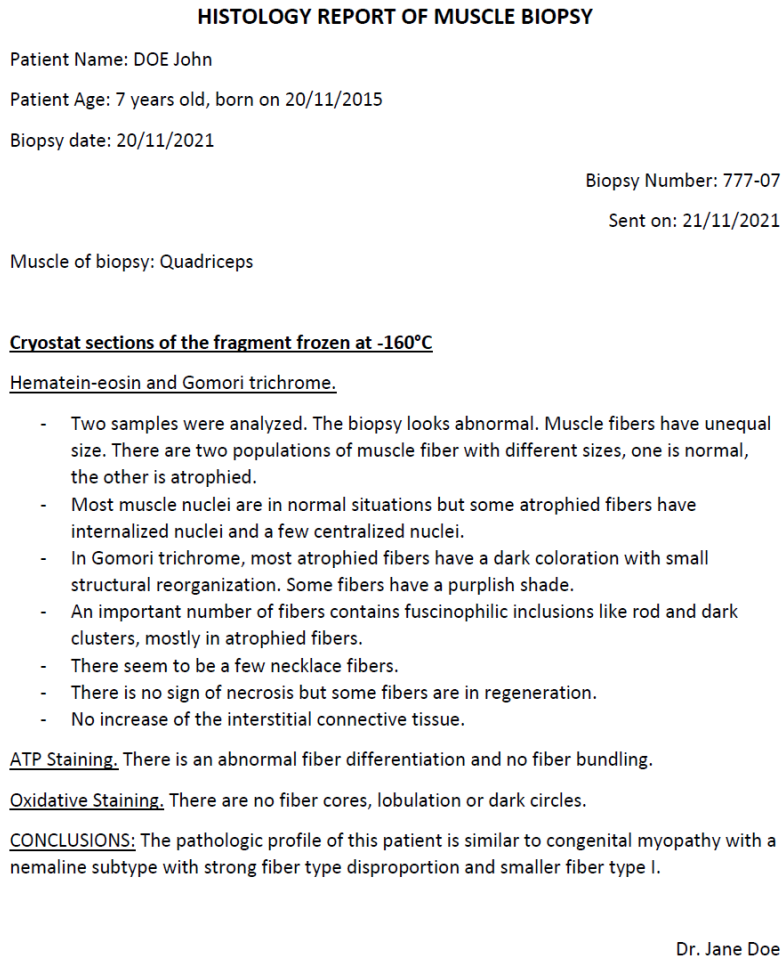
\includegraphics[width=0.85\textwidth]{figures/pdf_biopsie.png}
 \caption[Compte rendus de biopsie fictif]{\textbf{Exemple de compte rendu de biopsie fictif}}
 \label{fig:factice_report}
\end{figure}

Pour extraire les informations, nous avons comparé deux modèles présentés dans le chapitre 4 "Matériels et méthodes": un modèle performant et accessible uniquement via l'\gls{api} commerciale OpenAI (GPT-3.5-turbo) et un modèle autohébergé libre et open source \textit{Vicuna-7B}. Les résultats de l'extraction d'information présentés dans le tableau \ref{tab:json_data} montrent que le modèle d'\textit{OpenAI} GPT-3.5-turbo est capable d'extraire l'ensemble des informations demandées de manière satisfaisante sans erreurs tout en étant capable de détecter l'absence de certaines informations. Concernant le modèle \textit{Vicuna-7B}, qui a l'avantage d'être autohébergé et donc d'être utilisable pour des données sensibles, les performances sont moindres. En effet, six données sur treize ont été extraites correctement (nom, date de naissance, muscle, numéro de biopsie, diagnostic, anomalie PAS). Cependant, sept autres informations demandées ont été loupées par le modèle indiquant simplement "N/A".

Il est important de noter qu'en termes de ressources de calcul et de temps d'inférence, \textit{GPT-3.5} possède un avantage non négligeable, car ce modèle n'est accessible que par une \gls{api}. Les coûts de calcul pour l'application sont donc nuls et la requête ne prend que quelques secondes à être réalisée. Pour \textit{Vicuna-7B}, le modèle étant autohébergé, chaque requête requiert une quantité importante de ressources de calcul et monopolise ces ressources pour un temps important (environ 1min30 par document). Ces coûts en ressources et en temps de calcul couplés à une précision moindre, rendent difficile l'exploitation de modèle \gls{llms} génératif autohébergé pour la tâche d'extraction d'information à travers une interface en ligne. 

\textit{MyoExtract} est un outil qui peut permettre d'accélérer le processus de numérisation des comptes rendus de biopsie notamment dans \gls{impatient}. En effet, grâce à cette méthode de détection automatique, il est possible de préremplir les formulaires de numérisation des données dans \gls{impatient} en extrayant automatiquement les données de bases (âge, muscle, numéro de biopsies, anomalies de base...). Cette approche permet un gain de temps important, car il est alors possible d'extraire ces informations d'une masse de rapports sans travail manuel d'annotation, cette méthode apporte une solution aux soucis de mise à l'échelle d'\gls{impatient} dans le cadre de traitement d'une grande quantité de données.
\begin{table}[!ht]
\centering
\caption[Résultats de \textit{MyoExtract} pour \textit{GPT-3.5-turbo} and \textit{Vicuna7B}]{\textbf{Résultats de \textit{MyoExtract} pour GPT-3.5-turbo and Vicuna7B}. \textit{GPT-3.5-turbo} extrait l'ensemble des informations demandées de façon satisfaisant, tandis que \textit{Vicuna7B} n'en extrait que 6 sur 13.}
\label{tab:json_data}
\begin{tabularx}{\textwidth}{|l|X|X|}
\hline
\textbf{Information} & \textbf{GPT-3.5-turbo} & \textbf{Vicuna7B} \\ \hline
Nom & Pierre Laroche & Pierre Laroche \\ \hline
Âge & 24 & N/A \\ \hline
Date de naissance & 07-04-1994 & 07-04-1994 \\ \hline
Date de biopsie & 07-05-2018 & N/A \\ \hline
Date d'envoi & 12-06-2018 & N/A \\ \hline
Muscle & Quadriceps & quadriceps \\ \hline
N° Biopsie & 7377-07 & 7377-07 \\ \hline
Diagnostic & myopathie à némaline & myopathie à némaline avec forte disproportion des types de fibre \\ \hline
Anomalie PAS & yes & yes \\ \hline
Anomalie Soudan & no & N/A \\ \hline
Anomalie COX & N/A & N/A \\ \hline
Anomalie ATP & quasi-uniformité de type I & N/A \\ \hline
Anomalie Phospho. & N/A & N/A \\ \hline
\end{tabularx}
\end{table}

\section{\textit{MyoClassify}: un outil d'aide au diagnostic}
L'outil \textit{MyoClassify} a pour objectif de suggérer un diagnostic parmi les 3 types majoritaires de \gls{mc} (\gls{nm}, \gls{com}, \gls{cnm}) de manière automatique sur la base du texte du rapport de biopsie. Pour cela, nous avons utilisé comme jeu de données un corpus élargi de 192 rapports de biopsies fournis par l'institut de myologie de Paris labellisés selon 5 classes (tableau \ref{tab:number_patients}: \gls{nm}, \gls{com}, \gls{cnm}, diagnostic différent des 3 sous-types majoritaires (\textit{non-CM}) et pas de diagnostic final établi (\textit{UNCLEAR}).
\begin{figure}[!ht]
 \centering
 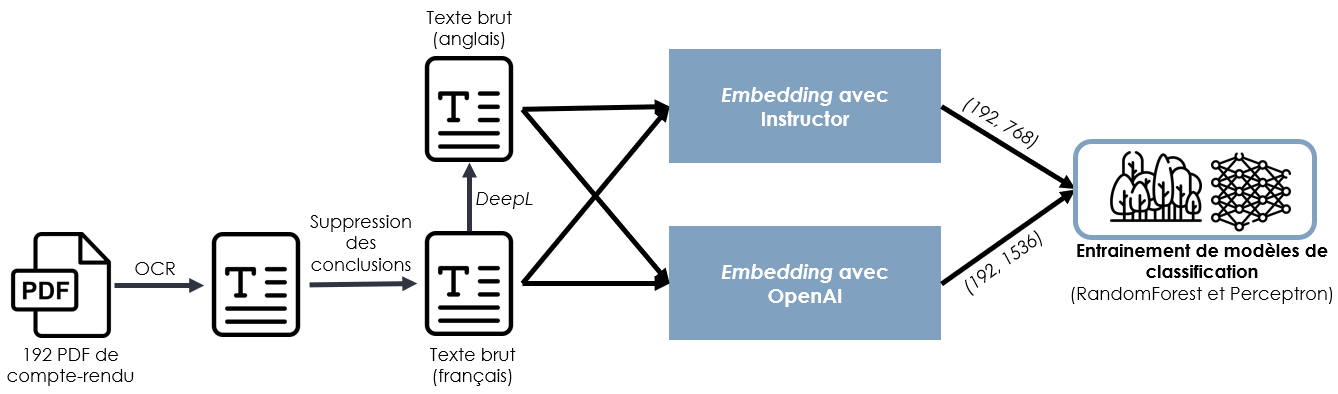
\includegraphics[width=1\textwidth]{figures/myoclassify_flow.png}
 \caption[Entraînement modèle \textit{MyoClassify}]{\textbf{Étapes de préparation et d'entraînement des modèles de \textit{MyoClassify}}}
 \label{fig:myoclassify_flow}
\end{figure}
\subsection{Méthodologie}
La figure \ref{fig:myoclassify_flow} représente l'ensemble des étapes réalisées pour préparer les données et entraîner un modèle de classification. Pour l'ensemble de ces rapports, nous avons réalisé une étape de détection de texte par \gls{ocr} avec \textit{Tesseract} (présenté dans le chapitre 4 "Matériels et méthodes" ainsi que dans le chapitre 5 sur \gls{impatient}). Ensuite, nous avons retiré les conclusions des rapports (indiquant la décision de diagnostic final, c'est-à-dire le label), afin que le modèle n'ait pas accès au diagnostic réel pour prédire le diagnostic. Enfin, à partir de ces conclusions, nous avons labellisé à la main chaque rapport avec un diagnostic parmi les 5 catégories listées ci-dessus.

Le contenu de chaque rapport (texte brut sans la partie conclusion) a été traduit en anglais grâce à l'\gls{api} DeepL afin de comparer les performances sur les textes anglais (traduit) et français (orignaux). Puis ces textes ont été encodés numériquement grâce à deux modèles\gls{llms} d'\textit{embedding} (présenter dans le chapitre 4 "Matériel et méthodes"): le modèle d'OpenAI (disponible uniquement \textit{via} \gls{api}) et le modèle \textit{Instructor-Large} (autohébergé). Les modèles d'\textit{embedding} sont des modèles qui prennent en entrée un texte (un mot, une phrase, un paragraphe ou un document) et qui produisent en sortie un vecteur numérique de grande taille capturant le sens sémantique du document d'entrée. Le modèle d'\textit{embedding} commercial d'OpenAI qui transforme les documents en vecteur de taille (1, 1536), tandis que le modèle auto hébergée libre et open source nommé \textit{Instructor-Large} qui transforme les documents en vecteur de taille (1, 768). Ces modèles sont des boites noires, c'est-à-dire que la signification des centaines (voire des milliers dans le cas d'OpenAI) de valeurs numériques décrivant le document n’est pas connue, cependant elles représentent le sens sémantique du texte.
À partir de ces 4 jeux de données (192 rapports dans 4 conditions: français/anglais et \textit{embedding} par OpenAI/Instructor), nous avons entrainé et comparé les performances pour la prédiction de diagnostic de deux algorithmes: les \textit{random forest} et les perceptrons (réseaux de neurones simples). Nous avons retiré du jeu de données les 54 rapports sans diagnostic, car ils ne peuvent pas être utilisés pour l'entraînement des modèles à apprentissage supervisé, ce qui aboutit à 138 rapports utilisés sur 4 labels différents pour l'entraînement des modèles (\gls{nm}, \gls{com}, \gls{cnm}, non-CM).
\begin{table}[!ht]
\centering
\caption[Nombre de comptes rendus de biopsies par diagnostic]{\textbf{Nombre de comptes rendus de biopsies par diagnostic}. Au total, ce sont 192 comptes rendus de biopsies répartis sur 5 labels différents, dont les 3 grands sous-types de myopathies congénitales (NM, COM, CNM), un label pour les comptes rendus sans diagnostics (UNCLEAR) et un label pour les comptes rendus non liés aux myopathies congénitales.}
\label{tab:number_patients}
\begin{tabular}{|l|c|}
\hline
\textbf{Diagnostic} & \textbf{Nombre de rapports} \\
\hline
Myopathie à Némaline (NM) & 44 \\
\hline
Myopathie à Cores (COM) & 48 \\
\hline
Myopathie centronucléaire (CNM) & 16 \\
\hline
Diagnostic non établi (UNCLEAR) & 54 \\
\hline
Autre (non-CM) & 30 \\
\hline
\end{tabular}
\end{table}

\subsection{Résultats des entraînements et performances des systèmes d'\textit{embedding}}
Au total, 8 conditions expérimentales pour la prédiction de diagnostics ont été évaluées: \textit{Embedding} OpenAI vs Instructor, rapports en Français vs traduits Anglais, \textit{Random Forest} vs Perceptrons (représenté en figure \ref{fig:myoclassify_flow}). Pour chacune des conditions expérimentales, les hyperparamètres des modèles ont été optimisés par grille et les performances ont été évaluées grâce à 10 cross-validations. Ceci a été fait pour (i) obtenir des modèles avec les meilleures performances possibles (optimisation par grille) et (ii) avoir une estimation robuste des performances (moyenne sur 10 essais par cross-validation). L'ensemble des résultats de ces entraînements (métriques de performances et modèles) sont disponibles en ligne à l'adresse: \url{https://wandb.ai/lambda-science/myo-text-classify/reports/MyoClassify-all-conditions-results--Vmlldzo0NDMyMTcw}.
\begin{table}[!ht]
\centering
\caption[Récapitulatif des performances des modèles \textit{MyoClassify}]{\textbf{Récapitulatif des performances des modèles \textit{MyoClassify}}. Pour chaque modèle, les valeurs d'exactitude, d'exactitude équilibrée, de score F1 pondéré et macro et de score F1 uniquement pour le classe CNM ont été mesurées.}
\label{tab:myoclassify_metrics}
\begin{tabularx}{\textwidth}{|X|c|c|c|c|c|}
\hline
\textbf{Nom} & \textbf{Exactitude} & \textbf{Exact. Equi.} & \textbf{F1 pond.} & \textbf{F1-Macro} & \textbf{F1 CNM} \\\hline
Instructor FR RF & 0.65 & 0.56 & 0.62 & 0.54 & 0.11 \\ \hline
Instructor EN RF & 0.67 & 0.54 & 0.62 & 0.52 & 0.00 \\ \hline
Instructor FR MLPC & 0.67 & 0.57 & 0.66 & 0.56 & 0.08 \\ \hline
Instructor EN MLPC & 0.64 & 0.58 & 0.64 & 0.58 & 0.32 \\ \hline
Openai FR RF & 0.61 & 0.56 & 0.60 & 0.58 & 0.45 \\ \hline
Openai EN RF & 0.65 & 0.5792 & 0.64 & 0.60 & 0.40 \\ \hline
Openai FR MLPC & 0.64 & 0.6 & 0.64 & 0.61 & 0.54 \\ \hline
\textbf{Openai EN MLPC} & \textbf{0.70} &\textbf{0.67}& \textbf{0.69} &\textbf{ 0.68} & \textbf{0.64} \\ \hline
\end{tabularx}
\end{table}
\begin{figure}[!ht]
 \centering
 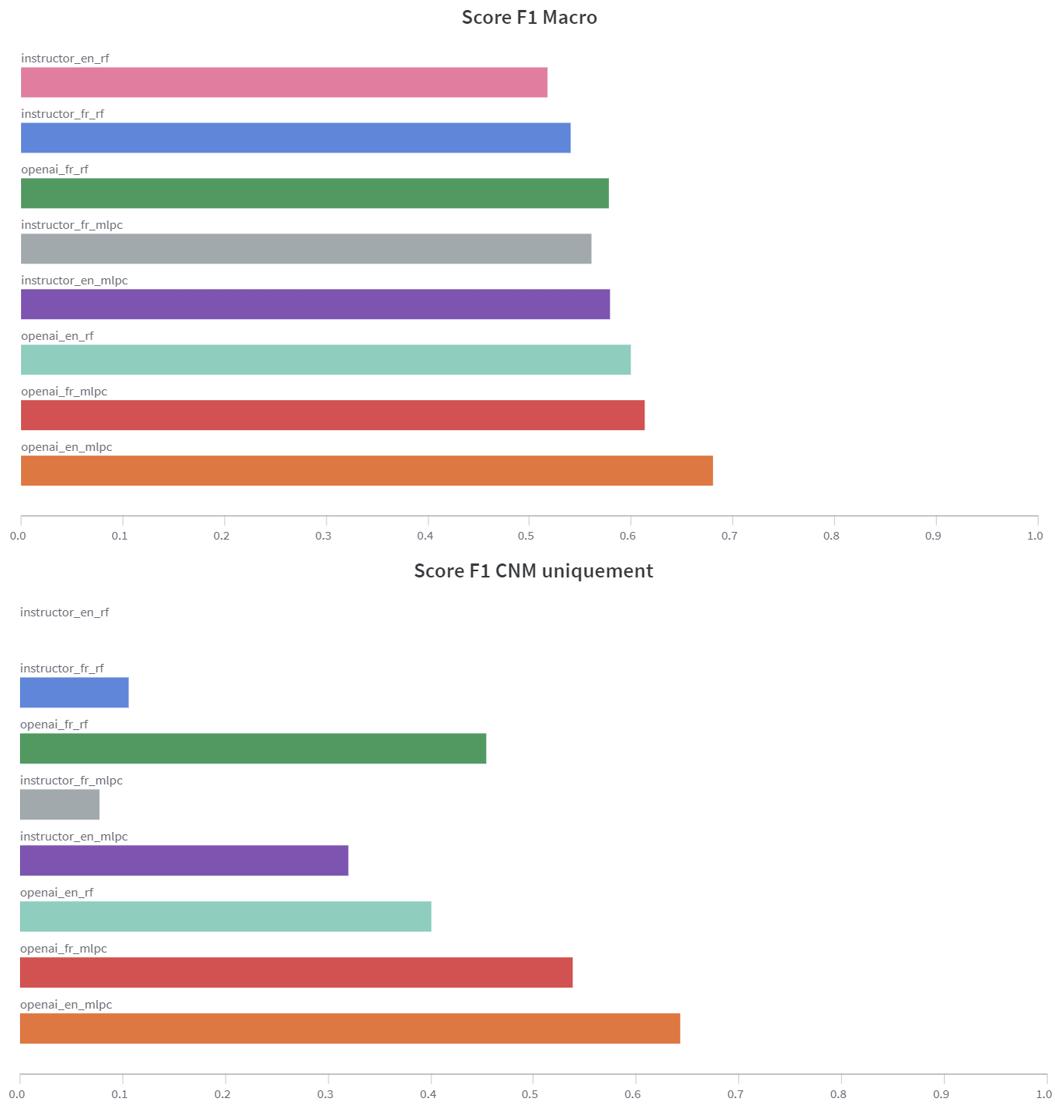
\includegraphics[width=1\textwidth]{figures/histo_myoclassify.png}
 \caption[Histogrammes des performances des modèle MyoClassify]{\textbf{Histogrammes des performances des modèles \textit{MyoClassify}} pour le score F1-macro (haut) et le score F1 pour la classe minoritaire (CNM) uniquement (bas). Globalement, le modèle le plus performant est le modèle \textit{OpenAI\_EN\_MLPC} pour les deux métriques présentées.}
 \label{fig:myoclassify_histo}
\end{figure}
\begin{figure}[!ht]
 \centering
 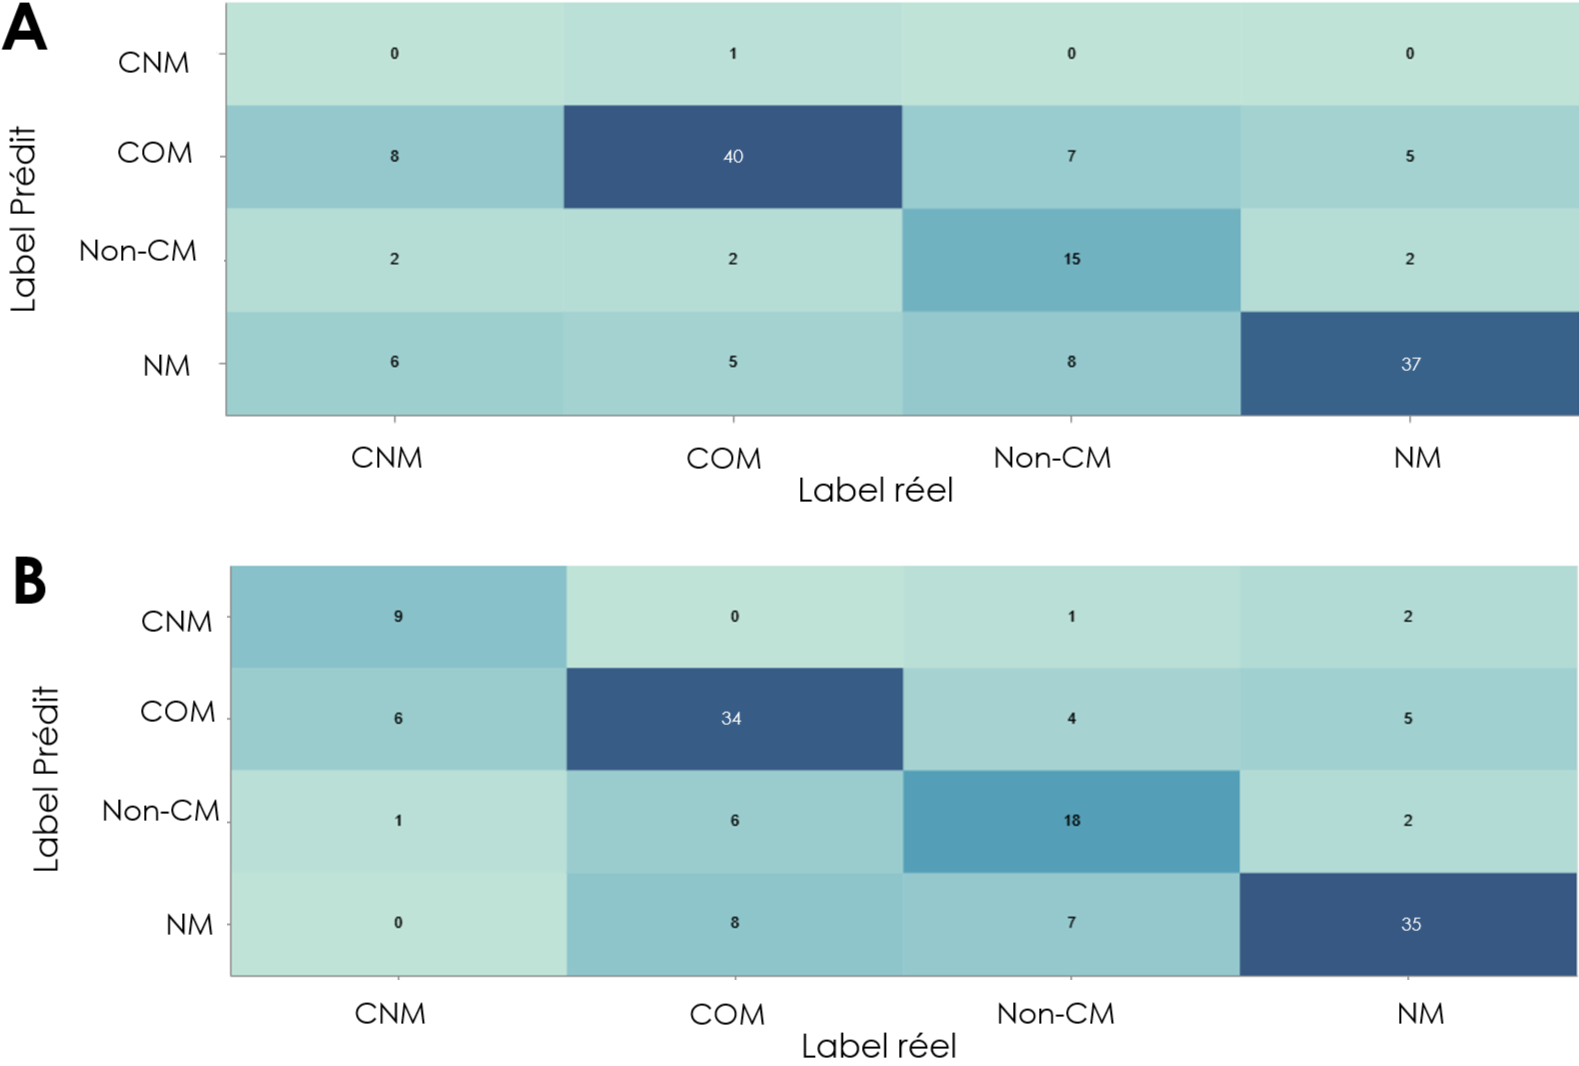
\includegraphics[width=1\textwidth]{figures/matrix_conf_myoclassify.png}
 \caption[Matrice de confusion \textit{MyoClassify}]{\textbf{Matrice de confusion des modèles} \textit{\textbf{MyoClassify}} pour le moins bon (\textit{instructor\_en\_rf} en haut) et le meilleur modèle (\textit{openai\_en\_mlpc} en bas) en termes de score F1.}
 \label{fig:myoclassify_conf}
\end{figure}

Sur le tableau \ref{tab:myoclassify_metrics} et les figures \ref{fig:myoclassify_histo} et \ref{fig:myoclassify_conf} on observe que, globalement, les performances à travers les conditions en termes de score F1 sont situées dans un intervalle entre 0.51 et 0.68 et que donc toutes les méthodes ont réalisé des erreurs de prédiction. Les modèles entraînés sur la base du modèle d'\textit{embedding} autohébergé \textit{Instructor} ont de moins bonnes performances globales à travers toutes les conditions. Cependant si l'on observe la matrice de confusion (\ref{fig:myoclassify_conf}), on observe que le moins bon modèle \textit{Instructor} a obtenu de meilleures performances de classifications que le meilleur modèle \textit{OpenAI} pour les deux classes de myopathies majoritaires: \gls{nm} et \gls{com} (40 prédictions correctes contre 34 pour les \gls{nm}, et 37 prédictions correctes contre 35 pour les \gls{com}). Cela indique donc que les métriques de performances globales sont donc très influencées par les performances du modèle sur les \gls{cnm}.

Pour la classe minoritaire (les \gls{cnm} avec 16 rapports), les performances des modèles sont très faibles pour l'\textit{embedding} du modèle \textit{Instructor}. Par exemple, pour notre modèle \textit{Instructor\_FR\_RF}, aucune \gls{cnm} n'a été prédite (matrice de confusion \ref{fig:myoclassify_conf}). Le modèle \textit{OpenAI\_EN\_MLPC} quant à lui obtient de meilleures performances et a été capable de prédire 9 des 16 \gls{cnm}. 

Dans le cadre du modèle d'\textit{embedding} d'OpenAI, la traduction des rapports en anglais a permis d'obtenir de meilleures performances dans toutes les conditions. De même, l'utilisation d'un perceptron multicouche a permis d'obtenir de meilleures performances en termes de score F1 dans toutes les conditions par rapport à la \textit{random forest}.

En termes de performances brutes, il semble recommandable de: (i) traduire les comptes rendus en anglais (ii) d'utiliser le modèle d'OpenAI pour l'\textit{embedding} et (iii) d'entrainer un perceptron multicouche pour apprendre à différencier les diagnostics en fonction de la représentation numérique des rapports (\textit{embeddings}).

\section{\textit{MyoSearch}: un moteur de recherche de patients}
En utilisant les techniques d'\textit{embedding}  pour représenter un texte sous forme numérique en capturant son sens sémantique, il est alors possible de calculer un score de similarité entre une requête en texte libre et une masse de documents pour trouver le document le plus proche. Avec \textit{MyoSearch} nous avons créé un outil qui permet de faire des requêtes en texte libre parmi l'ensemble des rapports de biopsies de patients. Il est alors possible de chercher rapidement chez quels patients un symptôme ou diagnostic particulier est présent. Cette création de moteur de recherche est totalement automatique et ne nécessite aucun travail d'annotation, contrairement à l'annotation de comptes rendus dans \gls{impatient}. Elle se déroule en deux phases: (i) l'intégration des données pour constituer la base de données puis (ii) la phase de requêtage de la base de données en fonction de l'entrée de l'utilisateur.

\subsection{Intégration des rapports: création de la base de données de vecteurs}
\begin{figure}[!ht]
 \centering
 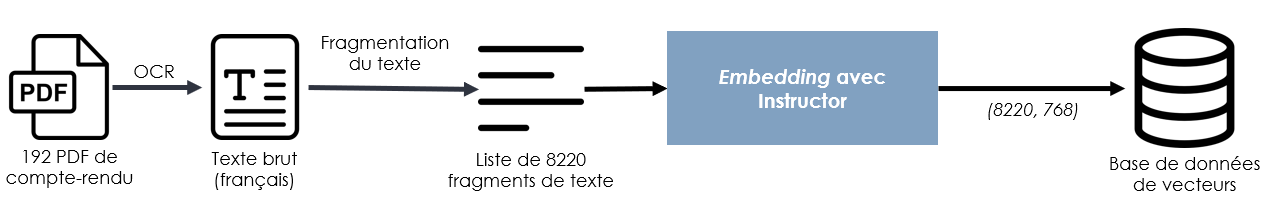
\includegraphics[width=1\textwidth]{figures/myosearch_ingest.png}
 \caption[Intégration des données dans \textit{MyoSearch}]{\textbf{Schéma de l'intégration des données pour le moteur de recherche \textit{MyoSearch}}. L'ensemble des comptes rendus de biopsie sont fragmentés et chaque fragment est transformé en vecteur numérique par le modèle d'\textit{embedding}. Chacune de ces représentations est intégrée dans la base de données de vecteurs.}
 \label{fig:myosearch_ingest}
\end{figure}

À la différence de \textit{MyoClassify}, cette fois-ci nous ne voulons pas générer 1 \textit{embedding} par document, mais plutôt séparer les documents en fragments et avoir un \textit{embedding} par fragment de document. Nous avons choisi de découper les documents en fragments de la taille d'une phrase et ainsi d'obtenir un \textit{embedding} pour chaque phrase du document. Ceci permet d'obtenir de meilleur résultat lors du requêtage de la base de données, car le sens sémantique de chaque phrase va pouvoir être comparé à la requête, plutôt que la moyenne de l'ensemble du document.

La figure \ref{fig:myosearch_ingest} présente la phase d'intégration des données. Nous avons d'abord détecté le texte des rapports PDF par \gls{ocr}. Comme cette détection est hétérogène et bruitée (images de texte dégradées, difficulté de reconnaissance des caractères), il est difficile de trouver les bornes exactes des phrases. Dès lors, nous avons à fragmenter le contenu en morceaux de taille maximale de 100 \textit{tokens} (environ 15 à 30 mots français) avec un recouvrement de 50, soit la taille moyenne d'une phrase en français. Pour 192 rapports, cela représente 8220 fragments de texte. Pour ces 8220 fragments, nous avons calculé leur représentation numérique (\textit{embedding}) et les avons intégrés dans une base de données de vecteurs. Enfin pour chaque fragment, il est possible d'ajouter des métadonnées qui peuvent servir de filtre pour les requêtes comme le diagnostic final ou le gène responsable de la maladie.

\subsection{Requêtage des données}
\begin{figure}[!ht]
 \centering
 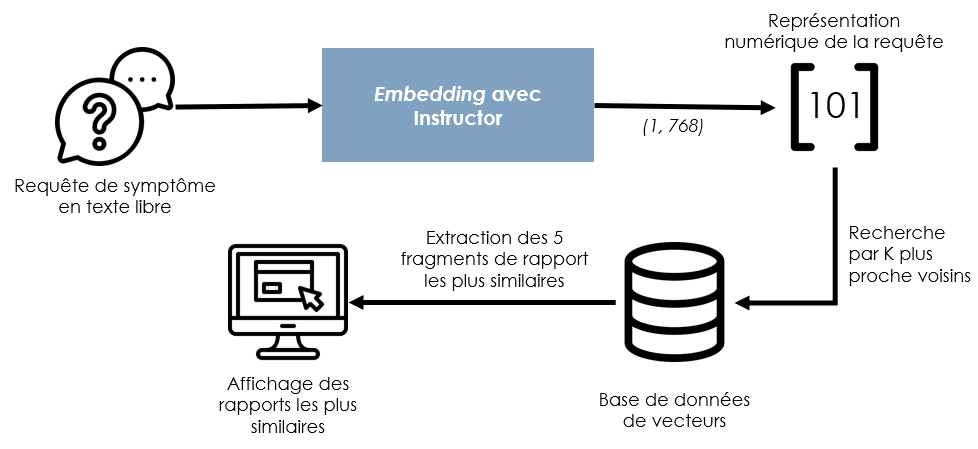
\includegraphics[width=1\textwidth]{figures/myosearch_query.png}
 \caption[Requêtage des données dans \textit{MyoSearch}]{\textbf{Schéma du requêtage des données dans \textit{MyoSearch}}. La requête formulée par l'utilisation est convertie en vecteur numérique qui est ensuite comparé (par similarité) à l'ensemble des fragments de comptes rendus intégré dans la base de données de vecteur.}
 \label{fig:myosearch_query}
\end{figure}
Quand l'ensemble des documents a été découpé et intégré dans la base de données, il est possible de réaliser des requêtes. La figure \ref{fig:myosearch_query} présente la phase de requêtage des données. L'utilisateur peut fournir \textit{via} l'interface web un symptôme d'intérêt en texte libre tel que "surcharge lipidique". Cette requête va ensuite être transformée en vecteur numérique par le modèle d'\textit{embedding }\textit{Instructor}. Ce vecteur va être comparé à la base de données de vecteurs pour rechercher les tops 5 plus proches voisins grâce à un algorithme nommé \textit{Hierarchical Navigable Small Worlds, HNSW}. Les cinq fragments avec les scores de similarité les plus élevés sont ensuite affichés sur l'interface web. Le tableau \ref{tab:myosearch_results} présente les résultats obtenus pour une requête dans MyoSearch. Par exemple pour la requête "surcharge lipidique" les trois rapports les plus proches font mention d'une surcharge en lipides chez des patients dont (i) le diagnostic n'est pas connu (ii) le diagnostic n'est pas une myopathie congénitale et (iii) chez un patient avec une \gls{nm}. Cette recherche est aussi multilingue, le modèle d'\textit{embedding} autorise des recherches entre une base de données française avec requête en anglais, ou inversement.
\begin{table}[!ht]
\centering
\caption[Exemple d'une requête et des résultats de \textit{MyoSearch}]{\textbf{Exemple d'une requête et des résultats de \textit{MyoSearch}}}
\label{tab:myosearch_results}
\begin{tabularx}{\textwidth}{|l|X|p{1cm}|p{2cm}|}
\hline
\textbf{Requête} & \textbf{Fragment le plus similaire} & \textbf{Rang} & \textbf{Rapport et diagnostic} \\\hline
"surcharge lipidique" & "d’inclusions. Il est à noter que l’on observe également une surcharge importante en lipides dans" \newline & 1 & 13405-105.txt UNCLEAR \\
 & "une myopathie congénitale. D'autre part, une surcharge importante en lipides qui nécessite"\newline & 2 & 11391-79.txt non-CM \\
 & "de surcharge en lipides - Technique de Koëlle : CONCLUSIONS : Anomalies caractéristiques d’une" & 3 & 5060-35.txt NM \\ \hline
\end{tabularx}
\end{table}

\section{Déploiement de l'outil}
Développé de façon \textit{open-source}, le code source de \gls{nlmyo} est disponible sur GitHub à l'adresse: \url{https://github.com/lambda-science/NLMyo} sous une licence AGPL-3 assurant le statut open source de l'outil. Une version de démonstration en ligne est déployée grâce à \textit{Streamlit} à l'adresse \url{https://lbgi.fr/NLMyo/}. Comme \gls{nlmyo} propose l'utilisation de \gls{llms} autohébergé, l'outil est hébergé sur un serveur avec un processeur 64 cœurs pour accélérer l'inférence du notre \gls{llms}. Si l'outil n'utilise que l'API OpenAI comme modèle génératif et d'\textit{embedding} alors il est possible d'héberger l'application sur un serveur nécessitant ainsi très peu de ressource de calcul.

\section{Discussions et perspectives de développement}
\gls{nlmyo} met à disposition des outils permettant le traitement de façon massive de rapports de comptes rendus médicaux et notamment des rapports de biopsie. Cependant, les défis pour rendre l'outil plus robuste sont multiples. 

Le premier défi concerne MyoSearch, le moteur de recherche de données de patients. Bien que la méthode soit fonctionnelle et novatrice, les résultats obtenus ne sont pas tout le temps similaire à la requête. Un travail d'amélioration des méthodes de fragmentation et de requêtage est nécessaire. De plus, il n'est actuellement possible que de chercher un symptôme à la fois, il faudrait créer un système permettant de croiser les résultats des requêtes pour plusieurs symptômes, permettant ainsi de chercher un profil de symptômes complet. De plus, l'ajout de métadonnées supplémentaires aux fragments (informations plus complètes sur le patient telles que le gène muté, l'âge, le muscle de la biopsie) sur les patients permettrait de réaliser des requêtes plus fines pour ne sélectionner, par exemple, que les patients liés à un gène en particulier.

Le second défi majeur concerne la protection de la confidentialité des données de santé. En effet, certains outils, pour obtenir les meilleures performances, reposent sur l'utilisation de \gls{llms} externes \textit{via} des l'\gls{api} OpenAI, ce qui est problématique dans le cadre de données sensibles, même anonymisées. Pour cela, nous avons aussi proposé une alternative avec un modèle autohébergé, mais pour l'instant celui-ci sous-performe. Par exemple dans \textit{MyoExtract}, les informations extraites sont incomplètes et dans \textit{MyoClassify} les scores d'exactitude et F1 sont globalement plus faibles, voire très faibles, pour la classe minoritaire (\gls{cnm}). Cependant, la recherche en terme de \gls{llms} est un domaine très dynamique et il est très probable qu'une solution autohébergée et performante soit disponible sous peu.